\section{More realistic bow shock models}
\label{sec:more-realistic-bow}

\begin{figure}
  \centering
  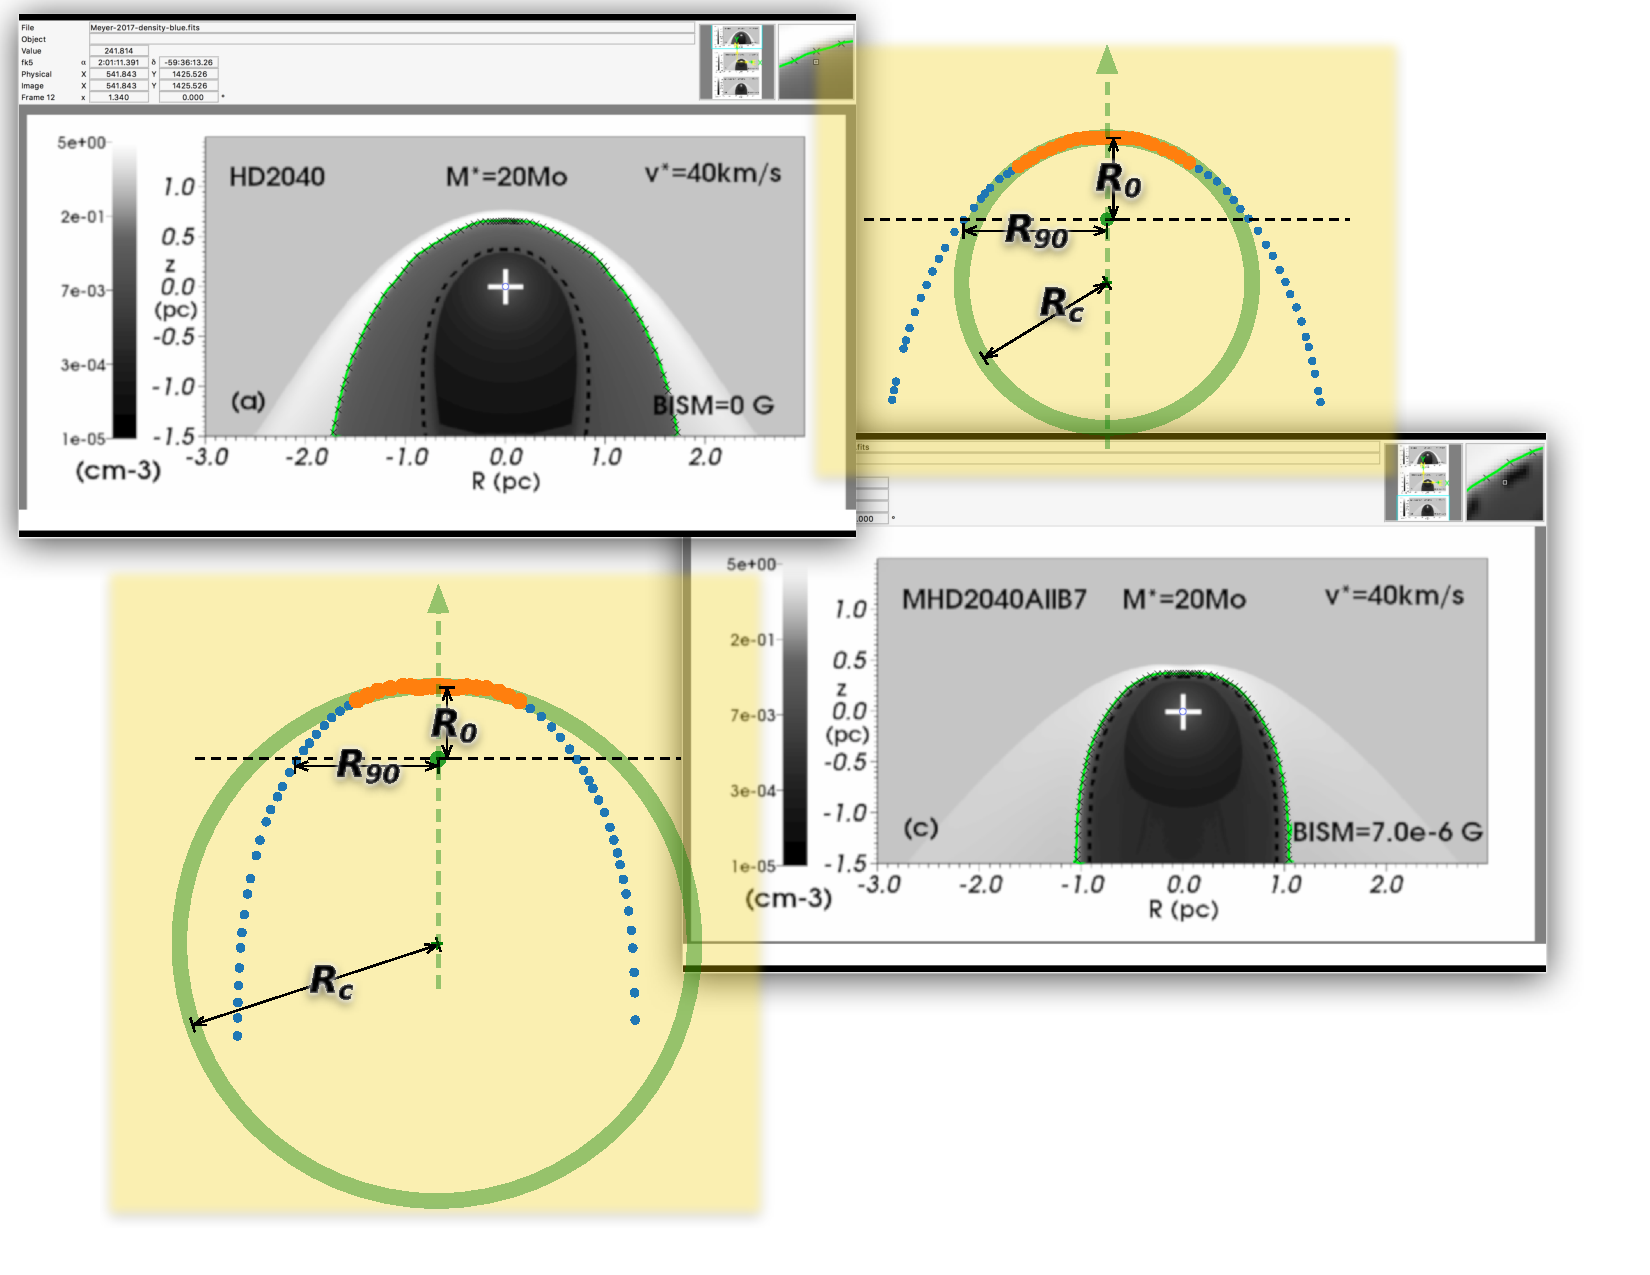
\includegraphics[width=\linewidth]{figs/M17-composite}
  \caption[]{Procedure for tracing the contact discontinuity from the
    \citet{Meyer:2017a} simulations.  The density maps from
    \citeauthor{Meyer:2017a}'s Fig.~3 are converted to FITS format and
    displayed using the software \textsc{SAOImage DS9}.  The density
    contour at \SI{0.4}{cm^{-3}} is displayed (shown in green in the
    figure) and this is traced by hand by placing ``point regions'' on
    the image (shown by black ``x'' shapes in the figure).  The zoom
    facility of the software allows the points to be placed with any
    required accuracy.  The points are saved to a file in the DS9
    region file format, which is then read by Python programs for
    further processing.  For example, the yellow boxes show circle
    fits and determination of the parameters \(R_0\), \(R_c\), and
    \(R_{90}\).  In this example, only the points shown in orange
    (within \ang{60} of axis) are used in the fits.}
  \label{fig:meyer-trace}
\end{figure}


\begin{figure}
  (a)\\
  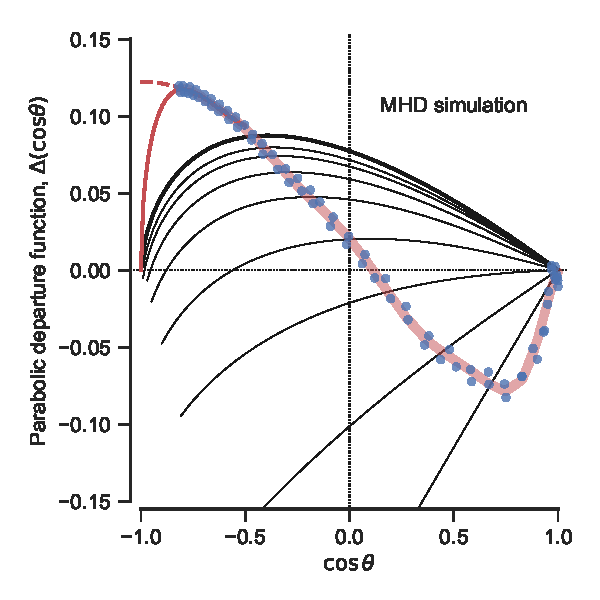
\includegraphics[width=\linewidth]
  {figs/depart-cheby-M17-MHD2040-AllB7}\\[-\baselineskip]
  (b)\\
  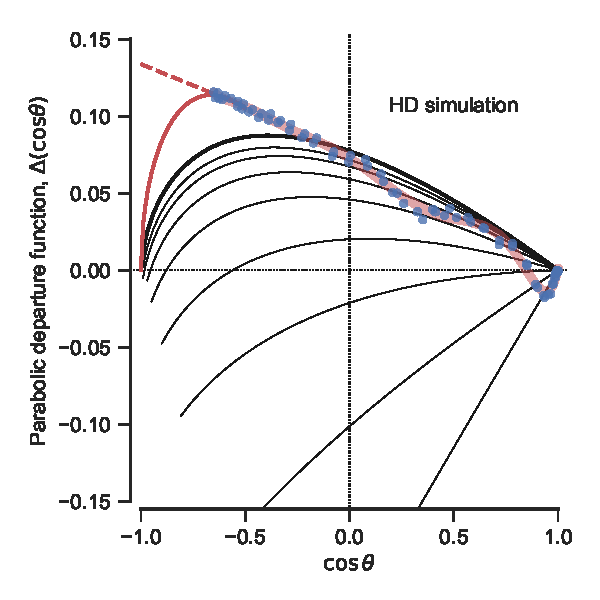
\includegraphics[width=\linewidth]
  {figs/depart-cheby-M17-HD2040}\\[-\baselineskip]
  \caption[]{Departure function for the shape of the contact
    discontinuity, measured from two numerical simulations of a
    \SI{20}{M_\odot} main-sequence star, moving at \SI{40}{km.s^{-1}}
    through a uniform medium of density \SI{0.57}{cm^{-3}}
    \citep{Meyer:2017a}. (a)~Magnetohydrodynamic simulation with
    ambient magnetic field of strength \SI{7}{\micro G}, oriented
    parallel to the stellar velocity. (b)~Hydrodynamic simulation with
    zero magnetic field.  Blue dots show the measured shape, while the
    thick, pale-red line shows a 12th-order Chebyshev polynomial fit.
    The published shapes only extend to
    \(\theta \approx 130\)--\ang{150}, so we extrapolate the shapes out to
    \(\theta = \ang{180}\). Two different extrapolations are shown,
    corresponding to bows that are asymptotically closed (dashed red
    line) or open (solid red line).  For comparison, black lines show
    the departure function for wilkinoid (thick line) and cantoids
    (thin lines).}
  \label{fig:sim-depart}
\end{figure}

The assumptions underlying the models of the previous section may
break down in various ways.  To test whether the planitude--alatude
analysis is still useful in less ``ideal'' situations, we here apply
it to more realistic simulations of stellar bow shocks.  We choose a
pair of hydromagnetic (HD) and magnetohydrodynamic (MHD) moving-star
simulations from \citet{Meyer:2017a}, in which the only difference is
the presence (MHD case) or absence (HD case) of an ambient magnetic
field with strength \(B = \SI{7}{\micro G}\), oriented parallel to the
stellar velocity.  In each case, the inner wind comes from a
\(20\,M_\odot\) main-sequence star, with mass loss rate and terminal
velocity that are roughly constant with time at
\(\dot{M}_{\w} \approx \SI{4e-7}{M_\odot.y^{-1}}\) and
\(V_{\w} \approx \SI{1200}{km.s^{-1}}\), while the outer wind is a
parallel stream due to the star's own motion at \SI{40}{km.s^{-1}}
through a uniform medium of density \SI{0.57}{cm^{-3}}.

For these parameters, the radiative cooling distance for shocked
ambient gas in the bow is a significant fraction (\(\approx 10\%\)) of the
bow shock size, \(R_0\), tending to increase towards the wings, and
the radiative cooling in the shocked stellar wind is even less
efficient.  This represents a significant violation of the assumptions
behind the thin-shell models, since the total shocked shell thickness
is of the same order as \(R_0\).  Nevertheless, the emissivity of
several observationally important emission processes, such as
mid-infrared thermal dust emission and the optical H\(\alpha\) emission
line, is concentrated near the contact discontinuity,\footnote{%
  Note that, in the non-magnetic HD models, efficient thermal
  conduction leads to a thick layer of hot, thermally evaporated
  ambient material that separates the shocked stellar wind from the
  cool, dense shell of shocked ambient gas \citep[see \S~3.3
  of][]{Meyer:2014b}.  In this case, the contact discontinuity is
  taken to be the boundary between hot and cold ambient gas, as
  opposed to the \textit{material discontinuity} between shocked
  ambient gas and shocked wind gas.  In the MHD models, the thermal
  conduction is almost completely suppressed, so that the material and
  contact discontinuities coincide. } %
so it is reasonable to use this surface as a first approximation for
the shape of the bow.

We have traced the contact discontinuity in the two models, using the
procedure outlined in Figure~\ref{fig:meyer-trace}, and show results
for the parabolic departure function (see
\S~\ref{sec:parab-depart-funct}) as blue symbols in
Figure~\ref{fig:sim-depart}.  The MHD simulation shows a strongly
negative dip in the departure function close to the apex
(\(\cos \theta = 1\)), indicating a very flat shape.\footnote{%
  \citet{Meyer:2017a} speculate that this flatness may be the
  signature of the formation of a complex multiple-shock topology at
  the apex \citep{de-Sterck:1999a}.  For our purposes, the reason does
  not matter, merely that the magnetic and non-magnetic models predict
  markedly different shapes. } %
The HD simulation shows only a small negative dip in the departure
function at the apex, but otherwise approximately follows the
wilkinoid curve in the forward hemisphere.  In both cases the
departure function is more positive than the wilkinoid in the far
wings (\(\cos \theta < -0.5\)), but we do not have data for the full range
of \(\theta\), and so two different extrapolations for
\(\theta \to \ang{180}\) are shown.  In the first (dashed red line in
figure), we fit a low-order polynomial of \(\cos \theta\) to the points
with \(\cos \theta < -0.5\) and extend it to \(\cos \theta = -1\), which gives
an asymptotically closed shape.  In the second extrapolation (solid
red line in figure), we fit a polynomial that is multiplied by
\((1 + \cos\theta)^{1/2}\), which forces the departure function to zero at
\(\cos \theta = -1\), giving an asymptotically open shape, as with the
wilkinoid.  In a true steady state, the far wings should be
asymptotically open, but as \(\theta \to \ang{180}\) the flow times become
longer and longer, so that a bow shock with a finite age will be
closed.

\begin{figure}
  \centering
  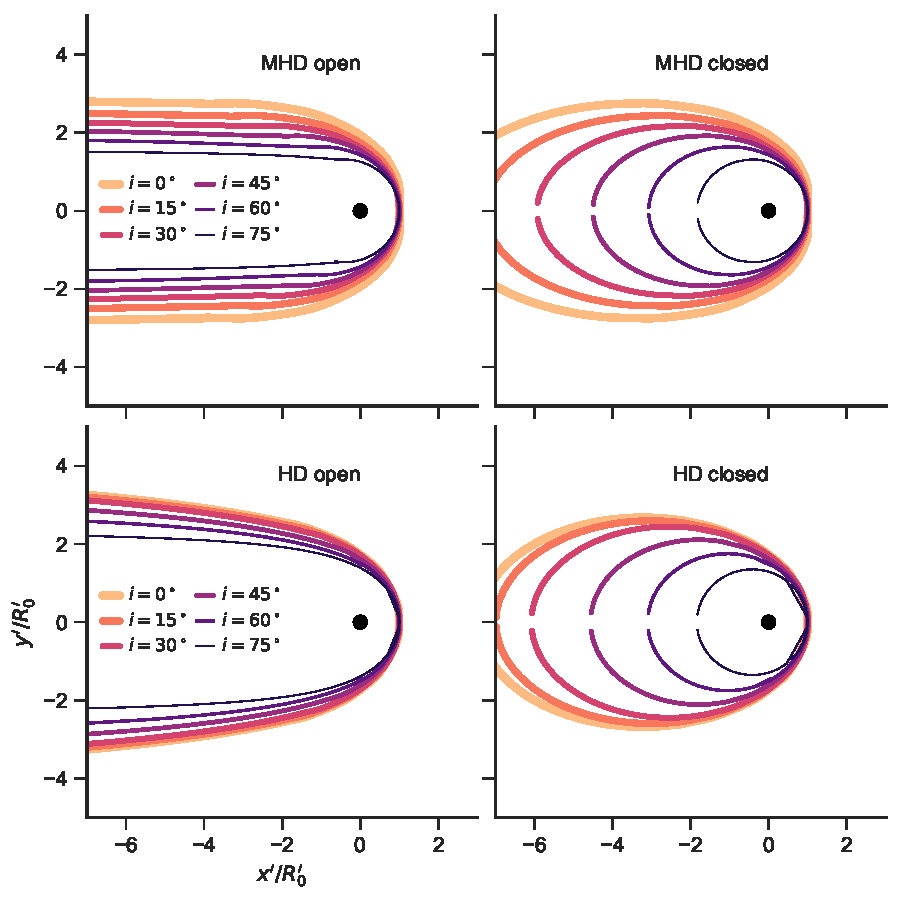
\includegraphics[width=\linewidth]{figs/test_xyprime_simulation}
  \caption[]{Projected shapes of contact discontinuity from
    simulations at different inclinations \(\abs{i}\) (varying line
    color and thickness, see key).  Top row shows magnetized
    simulation of Fig.~\ref{fig:sim-depart}a, bottom row shows
    non-magnetized simulation of Fig.~\ref{fig:sim-depart}b.  Left
    column shows asymptotically open extrapolation, right column shows
    asymptotically closed extrapolation.  All shapes are normalized to
    the projected apex distance, \(R_0'\) }
  \label{fig:sim-xyp}
\end{figure}

Using a 12th-order Chebyshev fit to the traced shapes, we show the
apparent shape of the contact discontinuity at a series of inclination
angles, \(\abs{i}\), in Figure~\ref{fig:sim-xyp}.  The four panels
show the two simulations for each of the two far-wing extrapolations.
Comparison with Figures~\ref{fig:xyprime}
and~\ref{fig:xyprime-ancantoid} shows the general tendency is the same
as with the wilkinoid: that the apex becomes less flat and the wings
less open as the inclination angle is increased.  There is no sign of
the sudden increase in openness at high inclination, as seen in the
cantoids and ancantoids that are asymptotically hyperbolic.  On the
other hand, the projected shapes of both simulations vary much more
strongly with \(\abs{i}\) than the wilkinoid does.  For the HD
simulation, this is mainly apparent for \(\abs{i} > \ang{30}\), but
for the MHD simulation it occurs at all inclinations.


\begin{figure}
  \centering
  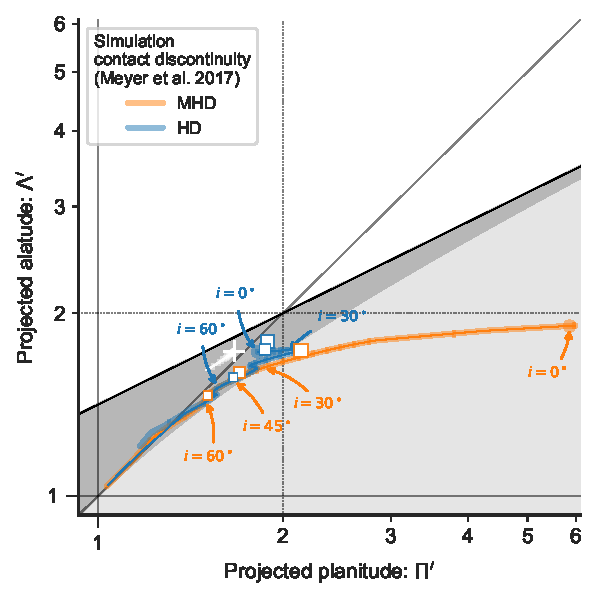
\includegraphics[width=\linewidth]{figs/m17-planitude-alatude}
  \caption[]{Apparent projected shapes of simulations in the
    \(\Pi'\)--\(\Lambda'\) plane.  Thick solid lines show the predicted
    inclination-dependent tracks of the traced contact discontinuity
    shape for the asymptotically open extrapolation, with tick marks
    indicating 20 equal intervals in \(\abs{\sin i}\). Thin solid
    lines show the same for the asymptotically closed extrapolation,
    which only deviates from the open case at the high-\(\abs{i}\) end
    of the HD tracks.  The true planitude and alatude are marked by
    filled circle symbols.  Open square symbols show the shapes traced
    from the dust emission maps at \SI{60}{\um} for inclinations of
    (largest to smallest) \ang{30}, \ang{45}, and \ang{60}. For
    comparison, the wilkinoid track is shown in white. Note that the
    scales of both axes are logarithmic in this case.}
  \label{fig:sim-Pi-Lambda}
\end{figure}

The resultant inclination-dependent tracks in the planitude--alatude
plane are shown in Figure~\ref{fig:sim-Pi-Lambda}.  These are compared
with measurements\footnote{%
  The shape measurements were performed by converting to contours the
  \SI{60}{\um} images in \citet{Meyer:2017a}'s Fig.~10 and then
  tracing the ridge of minimum radius of curvature of the contours.
  Identical results are found from using the \SI{100}{\um} maps
  instead.  For the \SI{25}{\um} maps, although the same results are
  found for low inclinations, in the maps with
  \(\abs{i} \ge \ang{45}\) in the HD case it becomes impossible to trace
  the limb-brightened rim because it becomes fainter than the emission
  from the true apex of the bow.} %
from post-processed infrared dust continuum maps at \SI{60}{\um}
\citep[\S~4.3 of][]{Meyer:2017a}, shown by open square symbols for
\(i = \ang{30}\), \ang{45}, and \ang{60}.  The agreement between the
two is good.  In particular, the \SI{60}{\um}-derived shapes are
always very close to the tracks derived from the contact discontinuity
shape. Also, the ordering of the three inclinations along the tracks
corresponds to what is predicted, although quantitatively there are
some slight deviations.  This close agreement stems from the fact,
emphasized by \citet{Meyer:2014b}, that the long-wavelength dust
emission from hot-star bow shocks tends to be dominated by material
just outside the contact discontinuity.  Note that there is almost no
difference in the planitude--alatude tracks between the closed and open
extrapolations.  This is because \(\Pi'\) and \(\Lambda'\) only depend on the
portion of \(R(\theta)\) between \(\theta_0\) (eq.~[\ref{eq:thetapar}]) and
\(\theta_{90}\) (eq.~[\ref{eq:th90}]), and these are both smaller than the
\(\theta\) range where extrapolation is necessary, except for in the HD
case at the highest inclinations.

\begin{figure}
  \centering
  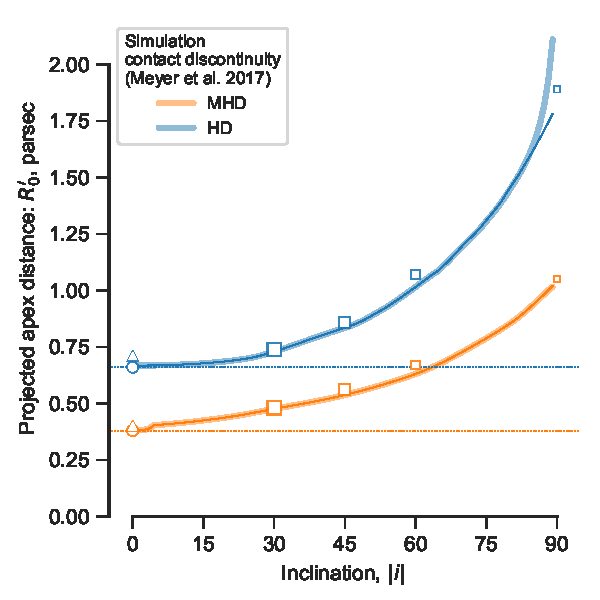
\includegraphics[width=\linewidth]{figs/m17-r0-prime}
  \caption[]{Apparent projected apex distance of simulations.  Line
    and symbol meanings are as in Figure~\ref{fig:sim-Pi-Lambda}.  In
    addition, triangle symbols at \(\abs{i} = \ang{0}\) denote radius
    measured on H\(\alpha\) optical emission maps.  Note that the distances
    for the blue square symbols have been adjusted according to the
    correction factor discussed in
    footnote~\ref{fn:meyer-correction}.}
  \label{fig:sim-R0-prime}
\end{figure}

Figure~\ref{fig:sim-R0-prime} shows the inclination
dependence of the projected apex distance, \(R_0'\).  As in the
previous figure, the lines show the prediction based on the shape of
the contact discontinuity, while the square symbols show the results
from the \SI{60}{\um} dust continuum maps.\footnote{%
  \label{fn:meyer-correction}
  There is an apparent error in the spatial scales for the HD
  simulations in Figs.~10 and 11 of \citet{Meyer:2017a}, with the dust
  emission peaks occurring at radii that are clearly too large.  The
  stated apex distance for the contact discontinuity in this
  simulation is \SI{0.69}{pc} from Table~2 of \citet{Meyer:2014b}, and
  the position of the peak in dust column density is \SI{0.70}{pc}
  from Fig.~17a of \citet{Meyer:2014b}.  These are consistent with
  Figs.~3, 4, and 7 of \citet{Meyer:2017a}, but not with Figs.~10 and
  11.  Luckily, the position of the true apex is clearly visible in
  the \SI{25}{\um} maps of Fig.~10 at inclinations of \ang{45} and
  \ang{60}.  The projected separation of the true apex is
  \(R_0 \cos i\), independent of the bow shape, which allows a
  correction factor of \num{0.65} to be found, assuming that the
  on-axis peak in the \SI{25}{\um} emission coincides with the peak in
  dust column density.  This correction has been applied to the blue
  square symbols shown in our Fig.~\ref{fig:sim-R0-prime}.} %
In addition, triangle symbols show results from H\(\alpha\) optical
emission line maps, which are given for \(i = 0\) in Fig.~7 of
\citet{Meyer:2017a}.  Again, the agreement is good between the values
derived from the shape of the contact discontinuity and those derived
from the surface brightness maps. The greatest discrepancy is seen
with the H\(\alpha\) maps and the intermediate inclination dust maps, with
\(R_0'\) being overestimated by a few percent in both cases.  The
differences in behavior between the two simulations are much larger
than this.  The larger true planitude of the MHD simulation means that
the relative increase of \(R_0'\) with \(\abs{i}\) is much stronger
than in the HD simulation for \(\abs{i} < \ang{45}\), as expected from
Figure~\ref{fig:quadric-projection}b.

\begin{figure}
  \centering
  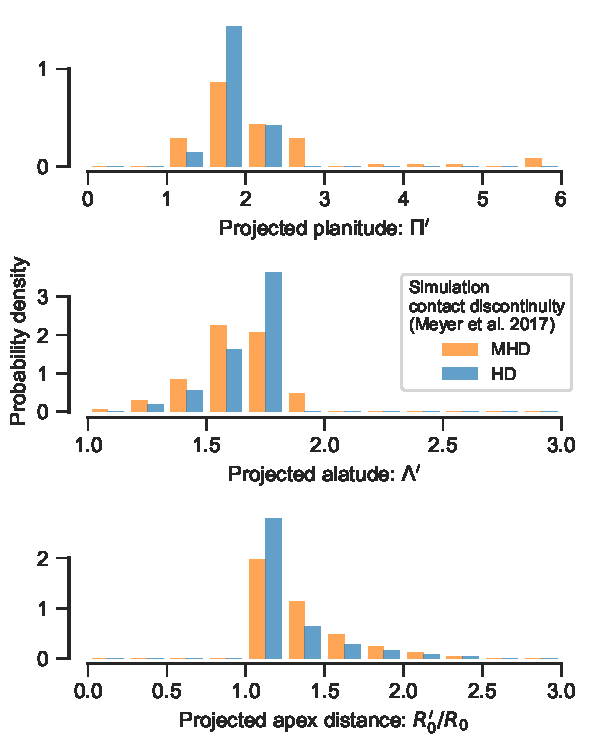
\includegraphics[width=\linewidth]{figs/m17-histograms}
  \caption[]{Histograms of (top to bottom) projected planitude,
    alatude, and bow shock size for the shape of the contact
    discontinuity in the \citet{Meyer:2017a} simulations. The \(y\)
    axis gives the probability density (per unit \(x\)-axis quantity),
    assuming a uniform distribution of viewing directions.}
  \label{fig:sim-histograms}
\end{figure}

The probability densities\footnote{%
  The probability density is defined so that its integral over the
  full range of the histogrammed variable is unity, making it
  independent of the histogram bin widths.  This means that the
  characteristic width of an approximately unimodal distribution is
  one over the maximum probability density.} %
of the apparent shape and size of the simulation bows (measured at the
contact discontinuity) are shown in Figure~\ref{fig:sim-histograms},
assuming that the viewing direction is uniformly distributed in solid
angle.  The modal value of the projected planitude is similar at
\(\Pi' \approx 1.8\) for both simulations, but the distribution is much
broader in the MHD case, which has a low-level wing extending out to
\(\Pi' \approx 6\).  The projected alatude distributions are both narrower
than the planitude (note the different scale of the histogram axis),
with the MHD case again being the broader of the two and peaking at a
slightly lower value (\(\Lambda' \approx 1.7\) as opposed to
\(\approx 1.8\) for the HD case).  Finally, the distribution of
projected-over-true apex distance is also broader for the MHD case. 


\begin{figure*}
  \centering
  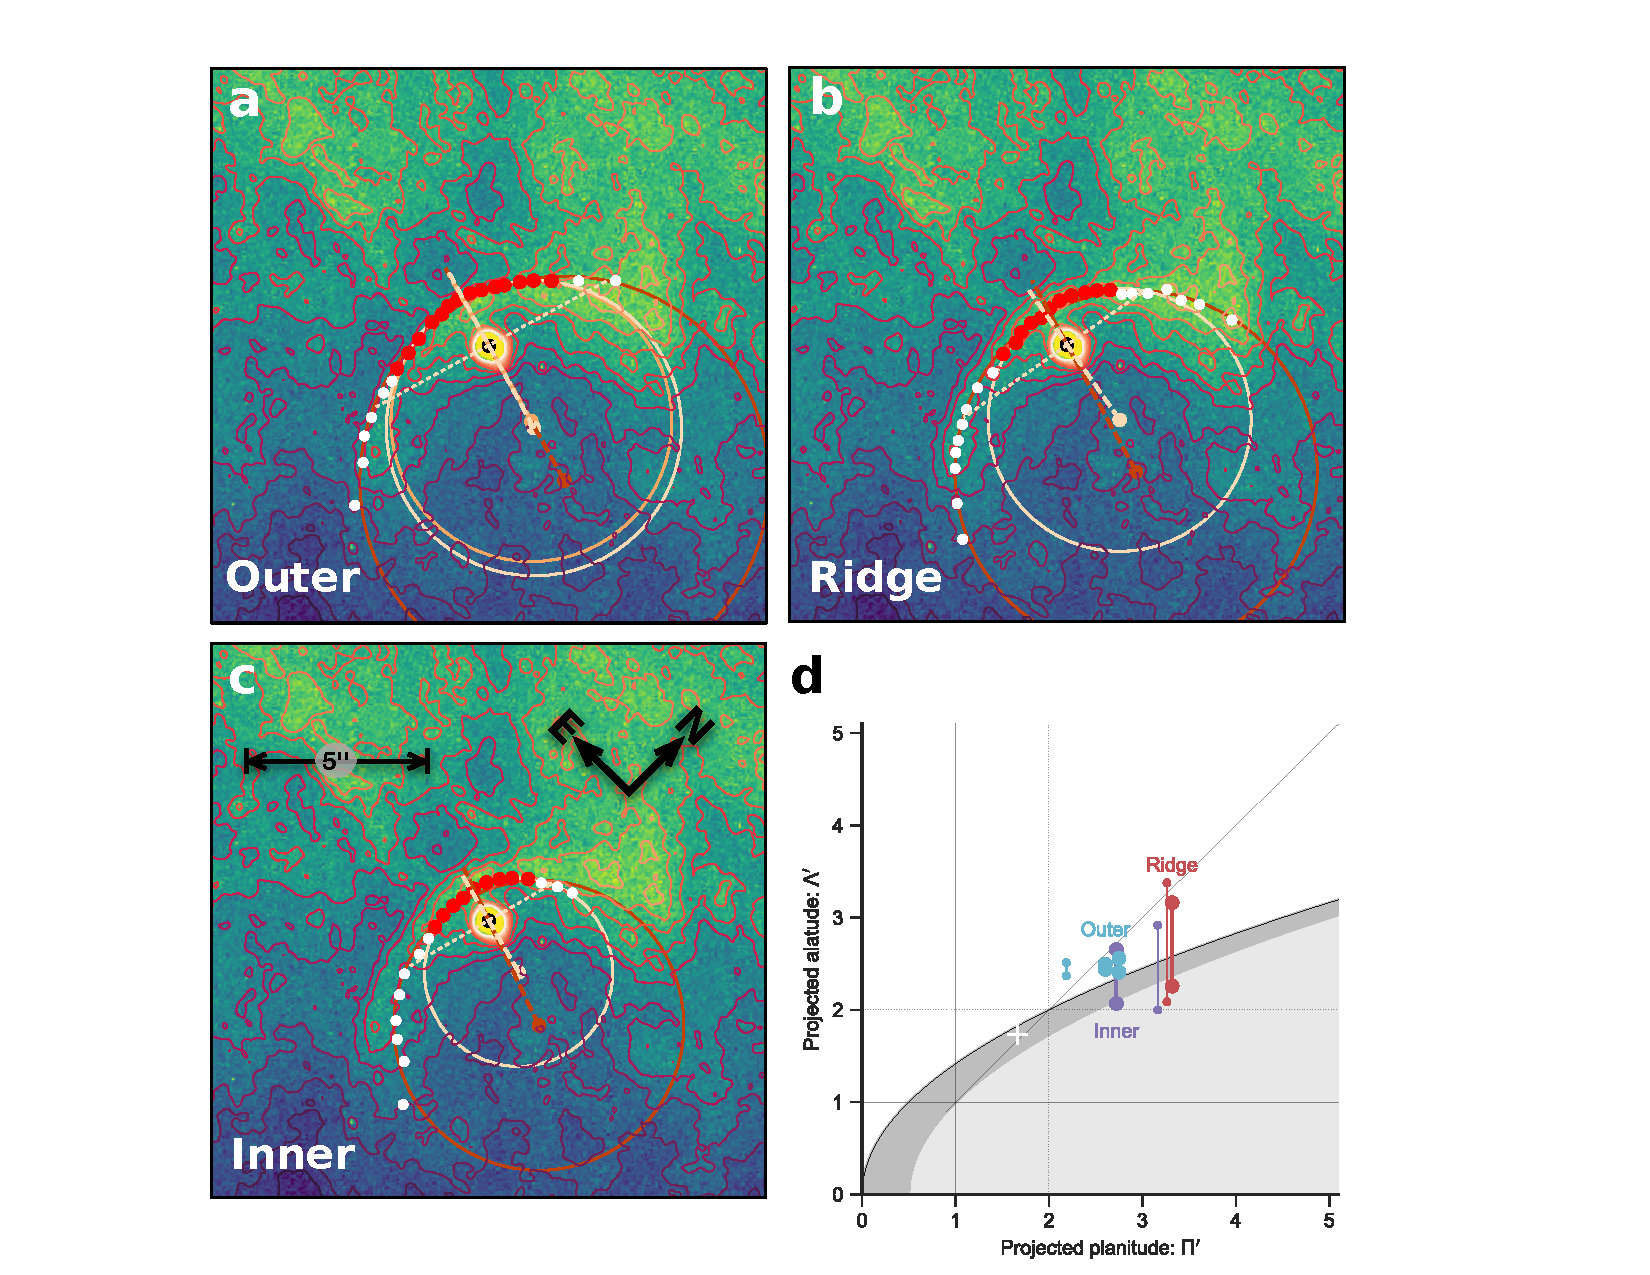
\includegraphics[width=\linewidth]{figs/new-000-400-multi-fig}
  \caption[]{Example empirical determination of planitude and alatude
    for an observed bow shock.  Color scale and contours show an
    \textit{HST} H\(\alpha\) image (ACS F658N filter,
    \citealp{Bally:2006a}) of M42~000-400. Three different bows have
    been traced by hand on the image (red and white filled symbols):
    (\textit{a})~inner edge, (\textit{b})~ridge of maximum emission,
    and (\textit{c})~outer edge.  For each panel, the dark-colored
    circle shows the initial fit to the full set of points (white and
    red), using the algorithm described in
    Appendix~\ref{app:rcurv-empirical}.  The center of curvature and
    derived axis are shown by a small filled circle and dashed line in
    the same color. Lighter colored circles show three subsequent
    iterations where the fit is restricted to points within
    \(\pm \Delta\theta = \ang{75}\) of the axis.  The subset of points used in
    the final iteration is marked in red.  The perpendicular radii for
    the final iteration are shown by dotted lines. In panels
    \textit{a} and \textit{b} the iterations converge immediately, but
    in panel \textit{c} the iterations stably oscillate between two
    slightly different solutions. }
  \label{fig:000-400-fit}
\end{figure*}

\begin{figure}
  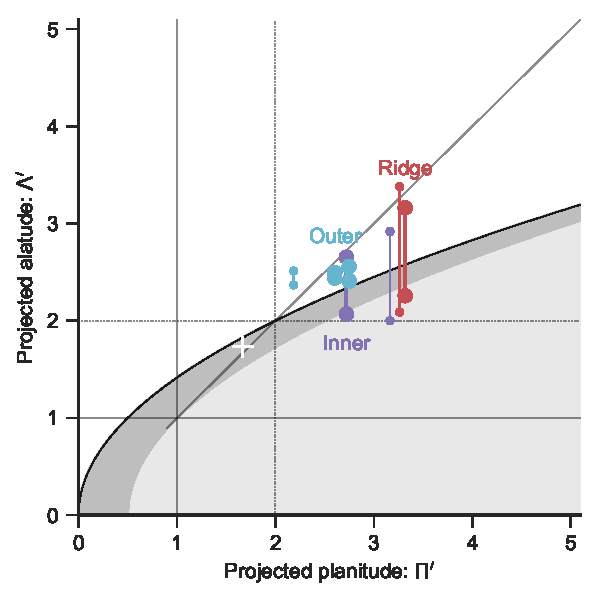
\includegraphics[width=\linewidth]{figs/000-400-planitude-alatude}
  \caption[]{Location in the projected planitude--alatude plane of the
    converged circle fits to the M42~000-400 bow.  For each solution,
    the two values of the alatude \(\Lambda'\), corresponding to
    \(R_{90}^+\) and \(R_{90}^-\), are joined by a vertical
    line. Large symbols show the results from the fits shown in
    Figure~\ref{fig:000-400-fit}, while small symbols show results for
    fits using \(\Delta\theta = \ang{60}\) instead of \ang{75}.}
  \label{fig:000-400-planitude-alatude}
\end{figure}

\begin{figure}
  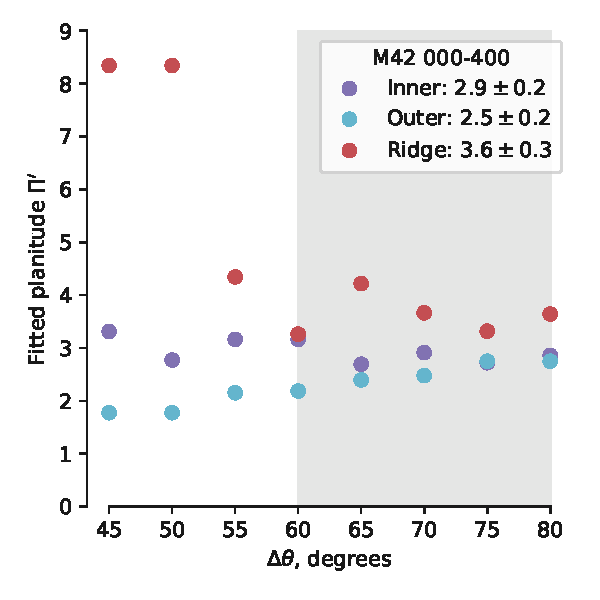
\includegraphics[width=\linewidth]{figs/000-400-Pi-vs-Dtheta}
  \caption[]{Sensitivity of fitted planitude to the parameter
    \(\Delta\theta\), which controls how close a point must be to the axis in
    order to be included in the circle fit. }
  \label{fig:000-400-Delta-theta}
\end{figure}

\section{Example application to observations}
\label{sec:obs}


As an example of measuring the projected planitude and alatude of a
real bow shock, we present an analysis of the H\(\alpha\) emission arc
associated with the proplyd M42~000-400 in the west of the Orion
Nebula \citep{Bally:2000a},\footnote{%
  The same object is listed as 4596-400 in some catalogs, such as
  \citet{Ricci:2008a}.  } %
which was used as an archetype of the bow shape in
Figure~\ref{fig:bow-terminology}.  To give an idea of the systematic
uncertainties and sensitivity to subjective choices, three different
tracings of the bow shape are considered (see
Fig.~\ref{fig:000-400-fit}): the peak of the emission arc (``ridge''),
and its inner and outer edges.  In all three
cases, we placed the points that define the bow by eye, using
SAOImage~DS9 in a similar fashion to in Figure~\ref{fig:meyer-trace},
and guided by the image contours.\footnote{%
  In the case of the ``ridge'' method at least, it is possible to
  automate this step, which we will discuss in detail in a following
  paper. } %
The principal hindrance to an accurate tracing of the bow shape in
this object is the strong and variable nebular background emission,
which particularly affects the far wing on the right hand side of the
image, where a bright background filament is superimposed on the bow.

We determine the planitude and alatude by fitting a circle to the
traced points within \(\pm \Delta\theta = \ang{75}\) bow axis, using the
iterative algorithm described in Appendix~\ref{app:rcurv-empirical}.
The fitted circle, when combined with the position of the central
source, yields the orientation of the bow axis, together with the apex
distance, \(R_0\), radius of curvature, \(R_\C\), and two
perpendicular radii (one for each wing), \(R_{90}^+\) and
\(R_{90}^-\).  These are all indicated on the panels of
Figure~\ref{fig:000-400-fit} by light-colored lines.\footnote{%
  For conciseness, we drop the prime symbol from the radii in this
  section and Appendix~\ref{app:rcurv-empirical}, even though all the
  quantities are projected ones.} %
The projected planitude and alatude then follow as \(\Pi = R_\C/R_0\),
\(\Lambda^+ = R_{90}^+/R_0\), \(\Lambda^- = R_{90}^-/R_0\), which are shown in Figure~\ref{fig:000-400-planitude-alatude}.

The planitude is found to have a moderate dependence on the choice of
\(\Delta\theta\), as shown in Figure~~\ref{fig:000-400-Dtheta}. The fact that
the radius of curvature is defined at a point (the projected apex)
might seem to argue for making \(\Delta\theta\) as small as possible, but that
leads to an extreme sensitivity of the circle fits to the exact
positions of the few points that are included in the fit.  A reliable
fit requires 4 or more points, which span a total separation
\(\approx R_\C\).

\section{Summary and discussion}
\label{sec:conc}

We have shown that the shapes of stellar bow shocks can be usefully
characterized by two dimensionless numbers: the \textit{planitude},
\(\Pi\), or flatness of the bow's apex, and the \textit{alatude},
\(\Lambda\), or openness of the bow's wings (\S~\ref{sec:plan-alat-bow}).
The planitude and alatude can be estimated from ratios of lengths that
can be straightforwardly measured from observations or theoretical
models.  We develop a general method (\S~\ref{sec:projection}) for
finding the projected shape, \((\Pi', \Lambda')\), of a bow shock's
limb-brightened edge, or \textit{tangent line}, as a function of
inclination angle, \(i\), where the emission shell is idealized as a
cylindrically symmetric surface.

We first apply this method to find inclination-dependent tracks on the
projected planitude--alatude plane for the special case of
\textit{quadric} surfaces (\S~\ref{sec:conic}), such as hyperboloids,
paraboloids, and spheroids, where the tangent line is a conic section.
The spheroids and hyperboloids occupy distinct regions of the plane,
with the paraboloids defining the boundary between the two.  As the
inclination is increased from \(\abs{i} = 0\) (side-on) to
\(\abs{i} = \ang{90}\) (end-on), the tracks first tend to approach the
diagonal \(\Lambda' = \Pi'\), corresponding to confocal conics, always
remaining within their own region.  At the highest inclinations, the
spheroids all converge at \(\abs{i} = \ang{90}\) on the point
\((\Pi', \Lambda') = (1, 1)\) and the paraboloids on the point
\((\Pi', \Lambda') = (2, 2)\).  The hyperboloids, on the other hand diverge as
\((\Pi', \Lambda') \to (\infty, \infty)\) for a finite
\(i_{\mathrm{crit}}\), which depends on the asymptotic opening angle
of the tail.  For \(\abs{i} > i_{\mathrm{crit}}\), the tangent line no
longer exists for the hyperboloid, and it would no longer appear to be
a curved bow shock.  We introduce the parabolic departure function
(\S~\ref{sec:parab-depart-funct}) as tool for visualizing differences
in bow shapes, \(R(\theta)\), over the full range,
\(\theta = [\ang{0}, \ang{180}]\).

We then apply the projection method to a set of thin-shell
hydrodynamic models of bow shocks (\S~\ref{sec:crw-scenario}): the
\textit{wilkinoid} from a wind-parallel stream interaction and the
\textit{cantoids} from wind-wind interactions.  We generalize the
latter to the \textit{ancantoids}, where one of the winds is
anisotropic.  We find that the wilkinoid is confined to a small region
of the \(\Pi'\)--\(\Lambda'\) plane, with projected planitude and alatude
varying with inclination by \(< 15\%\).  The cantoids and ancantoids
with sufficiently small values of \(\beta\), the wind momentum ratio, have
more interesting behavior, with tracks that pass from the spheroid
region at low inclinations to the hyperboloid region at high
inclinations.

Finally (\S~\ref{sec:more-realistic-bow}), we test the projected shape
analysis methods against the results of computational fluid dynamic
simulations of magnetized and non-magnetized bow shocks from
\citet{Meyer:2017a} of a runaway OB main-sequence star.  We find that
measurements made on maps of infrared dust emission can be accurate
diagnostics of the projected shape of the contact discontinuity for
this type of bow shock (Fig.~\ref{fig:sim-Pi-Lambda}).  The
distributions of projected planitude and alatude for a population of
randomly oriented bow shocks shows systematic differences between the
different simulations.

This paper is the first of a series that will apply our shape analysis
to a wide variety of models and observations of stellar bow shocks.
In a second paper, % \citep{Henney:2018a}
we consider the alternative model of dusty radiation-driven bow wave
\citep{Ochsendorf:2014a}, instead of a hydrodynamic bow shock, and
also calculate the signature in the planitude--alatude plane of
oscillations in the bow shape, which may be due to instabilities or a
time-varying source.  In a third paper, % \citep{Henney:2018b},
we apply our techniques to observational datasets for three different
classes of stellar bow shocks: OB stars \citep{Kobulnicky:2016a}, cool
giants/supergiants \citep{Cox:2012a}, and young stars in the extended
Orion Nebula \citep{Henney:2013a}.  In a fourth paper,
% \citep{Tarango-Yong:2018b},
we analyze the proplyd bow shocks in the core of the Orion Nebula
\citep{Garcia-Arredondo:2001a}.


%and was applied to the proplyds in the core of the ONC.
%We started measuring the projected characteristic radii $(R'_0,R'_c)$ for each proplyd in our
%sample and compare them with the ``conic equivalent'' of a two winds interaction model based 
%on \CRW{} work to estimate the intrinsic bow shock shape and get the ionizing flux for ionization balance 
%and the stagnation pressure for our sample of proplyds.
%Most results are consistent with a proplyd's photoevaporated flow with an anisotropic density
%distribution, with different anisotropy degrees. We ound that LV4 has the least anisotropic flow,
%while LV2 has the most anisotropic flow. And for the 177-341, 169-348 and 180-331 we found out that 
%the stellar wind is not enough to keep their bow socks stationary.

%%% Local Variables:
%%% mode: latex
%%% TeX-master: "quadrics-bowshock"
%%% End:
